\section{Nonmonotonic Rule Learning}\label{sec:nmrulelearn}

Previously described approaches learn Horn rules only, which, might not be sufficiently expressive to capture
exceptional cases. Therefore, they may predict erroneous facts~\cite{rumis}. For example, recalling $r_1$:
\[r_1 : \mi{livesIn(Y,Z)} \leftarrow \mi{married(X,Y)},\ \mi{livesIn(X,Z)} \]
If $r_1$ is applied on KG shown in Figure~\ref{rdf}, it will predict the incorrect fact $\mi{livesIn(alice,berlin)}$, which contradicts the exiting fact $\mi{livesIn(alice, amsterdam)}$. 

In contrast, nonmonotonic rules are capable of capturing the patterns for which it may be inaccurate to predict some facts (\ie exceptional cases); thus, preventing such predictions. For example, if $r_1$ can be adapted into a nonmontonic form to handle the cases where married couples may not live together, according to the KG in Figure~\ref{rdf}, that should be when one of them is a researcher; leading to new rule:
\[r'_1 : \mi{livesIn(Y,Z)} \leftarrow \mi{married(X,Y)},\ \mi{livesIn(X,Z)}, \naf \mi{researcher(Y)}\]
When the revised rule $r'_1$ is applied on the KG, it will not predict $\mi{livesIn(alice,berline)}$. 

In this section, we are discussing the different approaches for learning nonmonotonic rules from the data.


\subsection{Traditional Nonmonotonic Rule Learning}
Several approaches was introduced to extend Horn ILP into richer nonmonotonic logic formalisms such as~\cite{DBLP:conf/ijcai/InoueK97,DBLP:journals/tocl/Sakama05,R08,CorapiRL10,ILASP_system}. Once ILP programs are extended to nonmonotonic programs, they are interpreted under the answer set semantics explained in Section~\ref{sec:reasoning}~\cite{Shakerin2018}.

%These methods rely on CWA and focus on describing a dataset at hand where both positive and negative examples (\ie true and false facts respectively) are known, or can be safely determined.   

\leanparagraph{Inductive approaches} One of the early attempts by~\cite{DBLP:journals/tocl/Sakama05} proposed algorithms to induce a categorical logic program given the answer set of the background knowledge and either positive or negative examples. In particular, given a single answer set, they induce a program that has this answer set as a stable model for the learned program. In~\cite{Sakama2009}, the approach was extended to learn from multiple answer sets by introducing brave induction, where the answer sets of the learned hypothesis and the background knowledge cover the positive examples. This approach accepts only one positive example as a conjunction of atoms, while It totally dismisses the negative examples. ILASP ~\cite{ILASP_system}, induces the hypothesis (\ie rule) from multiple positive examples using brave induction, while it ensures that the negative examples are cautiously entailed (\ie negative examples are excluded from all answer sets). The algorithm exhaustively searches the space of possible clauses to find one that is consistent with all examples and background knowledge. To make this search feasible, it restricts the learning only target predicate(s). 
%Cautious induction, the counterpart of brave induction, is also too restricted as it can only induce atoms in the intersection of all stable models~\cite{Shakerin2018}.


\leanparagraph{Abductive learning approaches} DROPS~\cite{CorapiRL10} maps the ILP problem into an abductive learning problem. The authors followed it with ASPAL~\cite{ASPAL} which introduces encoding ILP problems as ASP programs and exploits ASP solver to find the hypothesis via abductive search. 

XHAIL~\cite{XHAIL} uses a hybrid algorithm combining abduction, deduction, and induction stages to generate the hypothesis (\ie rules). The system takes a background theory, a set of examples (both positive and negative), and user-defined predicate declarations to constrain the search space as input and returns a set of hypotheses that entail the examples with respect to background theory as an output. To that end, XHAIL still suffers from the same infeasible search space problem facing ILASP~\cite{Sakama2009}. An enhanced version of XHAIL to solve scalability was introduced in~\cite{XHAIL_extended} 

\gad{I think adding examples for each system would not be informative and we may diverge from the relevant challenges }
\gad{If we have time we can add the example of XHAIL steps from~\cite{XHAIL_extended}}



\subsection{Nonmonotonic Rule Learning over Knowledge Graphs}
\leanparagraph{Challenges of exiting approaches} The traditional nonmonotonic inductive and abductive algorithms cannot be directly used on KGs for several reasons:
First, they are designed to work under CWA such that the negative examples are assumed to exist or can be safely inferred. However, real-life KGs follows OWA and the negative examples are not available. Furthermore, they cannot be obtained from, e.g., domain experts due to the huge size of KGs.
Second, they cannot scale enough to handle the huge size of the KGs~\cite{Shakerin2018}. 
Third, restricting the search for some predefined target predicates for learning is not practical because
it is not known which parts of the KG need to be completed. Still learning rules for all predicates appearing in the KG unfeasible due to the huge
size of KGs. Finally,
the definition of a language bias turns out to be cumbersome since the schema of the
KG is usually not available.

Recently, several approaches have been developed specifically to learn nonmonotonic rules from the large KGs, taking into account the OWA and the huge size of the KG.

\begin{figure}[t]
\centering
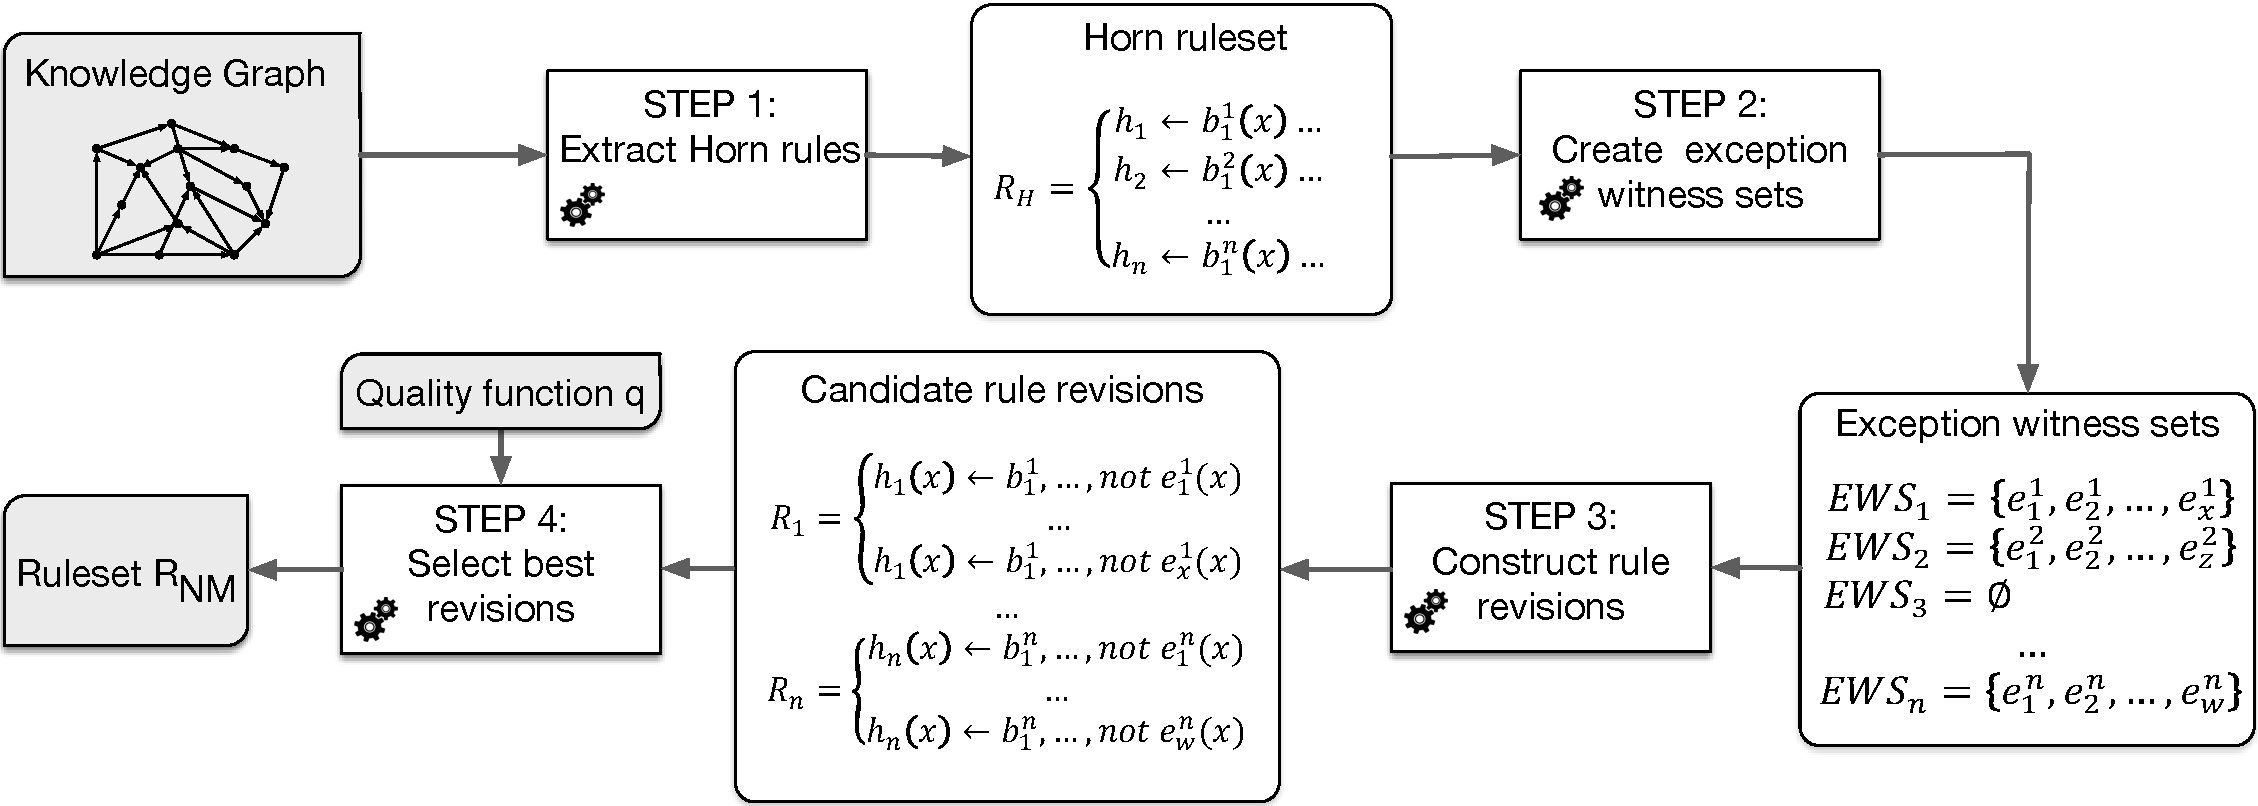
\includegraphics[width=\textwidth]{figures/overview}
\caption{Rule revision process by~\cite{gad2016,rumis}}
\label{fig:iswc_process}
\end{figure}
\leanparagraph{Program consistency maximization approaches} In both \cite{gad2016} and RUMIS~\cite{RUMIS} introduced an approach to revise a set of Horn rules $R_H$ learned from KGs into nonmonotonic set $R_{MN}$ by adding at most one negated atom to each rule. The final revision is chosen such that the average quality of the Horn rule set is maximized while the conflict between the predictions of the different rules are minimized. 

In order to estimate the conflict between the predictions of the rules, they introduce the notion of auxiliary rules, concretely, for a rule 
\[r:H \leftarrow B, \naf E\] an auxiliary version is \[r:\mi{not\_H} \leftarrow B, E\] where $\mi{not\_H}$ is a fresh predicate indicating that $H$ will not be derived by this rule. The number of grounded pairs $\tuple{H,\mi{not\_H}}$ in the answer set generated by the rule set and the KG indicates the degree of conflict.


Figure~\ref{fig:iswc_process} shows the rule revision steps as described by~\cite{gad2016} (and similarly RUMIS). 

First, Horn rules are extracted from the KG. In the case of~\cite{gad2016}, the KG is first projected from the binary relations into unary one by introducing new predicates that combines the original predicate and the class of the object part (aka propositionalization). For example, given facts $\mi{isMarriedTo(bob, alice)}$ and $\mi{researcher(alice)}$, the first can be projected into $\mi{isMarriedTo\_researcher(bob)}$. Using the class of the object instead of the instances allows learning patterns. A traditional item set mining approach to obtain the Horn rules $R_H$ from the projected KG. RUMIS takes as input a rule set learned by using any positive rule mining system such as ~\cite{amie,op,rdf2rules}.  

Second, in order to construct the exception witness set (EWS), for each rule $r$ the normal and abnormal  sets are defined: the normal set is the set of the substitutions of the variables $\mathcal{V}$ with the entities such that satisfy both the head and the body of the rule $r$, while the abnormal set contains the  substitutions for which the rule body is satisfied but not the head.

Formally, for each rule $r \in \cR_H$, let $\mathcal{V}$ be the set of variables of $r$, the normal and abnormal sets are respectively defined as follows:
\begin{itemize}
\item $NS(r, \cG) = \{\theta \mid head(r)\theta, body(r)\theta \subseteq \cG\}$
\item $ABS(r, \cG) = \{\theta \mid body(r)\theta \subseteq \cG , head(r)\theta \notin \cG\}$\\
where $\theta: \mathcal{V} \rightarrow \cC$.
\end{itemize}

\begin{example}
Consider the KG $\cG_1$ and $r_1$ as before, the normal set for $r_1$ is $NS(r_1,\cG_1)=\{\theta_1, \theta_2 ,\theta_3\}$, where $\theta_1 = \{X/brad, Y/ann, Z/berlin\}$,\\  $\theta_2 = \{X/john, Y/kate, Z/chicago\}$ and $\theta_3 = \{X/sue, Y/li, Z/beijing\}$.\\ and the abnormal set, $ABS(r_1,\cG_1)=\{\theta_4,\theta_5, \theta_6\}$, \\such that $\theta_4=\{X/bob, Y/alice, Z/berlin\}$,  $\theta_5=\{X/clara, Y/dave, Z/chicago\}$, and $\theta_6=\{X/mat, Y/lucy, Z/amsterdam\}$.
\qed
\end{example}

 \gad{stopped here! details to be added}
 
Second, based on the (ab)normal substitutions, let $\mathcal{X} \subseteq \mathcal{V}$, we compute the Exception Witness Set (EWS) for each $r \in \cR_H$, which is a maximal set of predicates $EWS(r,\cG,\mathcal{X}) = \{p_1,...,p_k\}$ s.t.:
\begin{itemize}
\item $\forall i \in \{1,..,k\} : \exists \theta \in ABS(r, \cG)\ s.t.\ p_i(\mathcal{X}\theta) \in \cG$, and 
\item $\forall \theta \in NS(r,\cG) :  p_1(\mathcal{X}\theta), ...,p_k(\mathcal{X}\theta) \notin \cG$
\end{itemize}



%
%\leanparagraph{RUMIS} RUMIS starts with a set of \textit{closed} Horn rules $\cR_H$, which can be learned by using any positive rules mining systems \cite{amie,op,rdf2rules}, and then finds the single best exception for each Horn rule $r \in \cR_H$ to obtain a revised set of nonmonotonic rules $\cR_{NM}$ such that the difference between $\cG^i$ and $\cG^i_{R_{NM}}$ is minimized. Below is the overview of how RUMIS revises the ruleset $\cR_H$ to achieve $\cR_{NM}$.
%\begin{enumerate}
%\item
% First, for each rule $r \in \cR_H$, let $\mathcal{V}$ be the set of variables of $r$, the normal substitutions and abnormal substitutions are respectively extracted as follows:
%\begin{itemize}
%\item $NS(r, \cG) = \{\theta \mid head(r)\theta, body(r)\theta \subseteq \cG\}$
%\item $ABS(r, \cG) = \{\theta \mid body(r)\theta \subseteq \cG , head(r)\theta \notin \cG\}$\\
%where $\theta: \mathcal{V} \rightarrow \cC$.
%\end{itemize}
%Informally, the normal and abnormal substitutions stand for the substitutions of variables $\mathcal{V}$ with the entities such that the rule $r$ holds (both the head and the body hold) and does not hold (only the body holds) in $\cG$, correspondingly.
%\begin{example}
%Consider the KG $\cG_1$ and $r_1$ as before, we have $NS(r_1,\cG_1)=\{\theta_1, \theta_2 ,\theta_3\}$, where $\theta_1 = \{X/brad, Y/ann, Z/berlin\}$, $\theta_2 = \{X/john, Y/kate, Z/chicago\}$ and $\theta_3 = \{X/sue, Y/li, Z/beijing\}$. Similarly, $ABS(r_1,\cG_1)=\{\{X/bob, Y/alice, Z/berlin\},$ $\{X/clara, Y/dave, Z/chicago\},$ $\{X/mat, Y/lucy, Z/amsterdam\}\}$.
%\qed
%\end{example}
%\item 
%Second, based on the (ab)normal substitutions, let $\mathcal{X} \subseteq \mathcal{V}$, we compute the Exception Witness Set (EWS) for each $r \in \cR_H$, which is a maximal set of predicates $EWS(r,\cG,\mathcal{X}) = \{p_1,...,p_k\}$ s.t.:
%\begin{itemize}
%\item $\forall i \in \{1,..,k\} : \exists \theta \in ABS(r, \cG)\ s.t.\ p_i(\mathcal{X}\theta) \in \cG$, and 
%\item $\forall \theta \in NS(r,\cG) :  p_1(\mathcal{X}\theta), ...,p_k(\mathcal{X}\theta) \notin \cG$
%\end{itemize}
Intuitively, $\mathcal{X}$ is set containing of either 1 or 2 variables of $\mathcal{V}$ corresponding to the usage of unary or binary exception. While the first condition ensures that the exception does affect the abnormal substitutions of the rule, the second condition ensures that it does not affect the rule's normal substitutions part. In other words, $EWS(r,\cG,\mathcal{X})$ contains all possible exceptions to be added to $r$ at variables of $\mathcal{X}$, such that the addition of the exception should result in the rule $r'$, satisfying $\textit{b-supp}(r', \cG) < \textit{b-supp}(r, \cG)$ and $\textit{r-supp}(r', \cG) = \textit{r-supp}(r, \cG)$. Intuitively, the application of exception should lead to the decrease of the body support, but not lead to the decrease of
the rule support, i.e., exceptions should explain the absence of predictions expected to be in the graph rather then their presence.
\begin{example}
We have $EWS(r_1,\cG_1,\{X\}) = \{artist\}$ and $EWS(r_1,\cG_1,\{Y\}) = \{researcher\}$.
\qed
\end{example}
Combining all possible exceptions at different variables of rule we have:
\[EWS(r,\cG) = \bigcup_{\forall\mathcal{X}\subseteq \mathcal{V}}EWS(r,\cG,\mathcal{X})\]

%\item 
For each rule $r \in \cR_H$, we now have $EWS(r,\cG)$ containing all of its exception candidates. The final step is to rank these exceptions based on some scoring function and select the one with the highest score to build the rule with exception $r'$ in $\cR_{NM}$. At this point, several exception scoring functions have been proposed by RUMIS \cite{rumis}.
%Let $r_i^j$ be the nonmonotonic rule built from $r_i \in \cR_H$ by adding $j$-th exception of $EWS(r_i,\cG)$, the introduced exception scoring functions are as follows:
\begin{itemize}
\item \textbf{Naive (N)}: is the simplest scoring function, which choosing the exception with the highest value of some standard rule measure $rm$. RUMIS system uses conviction as the rule measure $rm$.
\item \textbf{PM}: invoke the novel concept of \textit{partial materialization}. The idea behind it is to rank candidate exceptions not based on $\cG$ as in Naive, but rather on its
extension with predictions produced by other rules in $\cR_H$, thus ensuring a crosstalk between the rules.
\item \textbf{OPM}: stands for \textit{ordered partial materialization}. This exception scoring function is similar to \textbf{PM}, but also takes into account the order of rules in $\cR_{H}$, which is defined based on some rule measure (e.g. \textit{r-supp} in RUMIS).

\thi {Should I describe the 3 ranking measures in more detail?}
\end{itemize}
%\end{enumerate}





%\leanparagraph{Learning rules with external resources}